\section{Computer Vision}
La Computer Vision (ou vision par ordinateur) comprend l'acquisition, l'analyse et
le traitement des images numériques pour comprendre et extraire des données, informations
ou décisions.\\
Les applications et possibilités de ce domaine sont pour ainsi dire, infinie.

\subsection{Défis liés à la mesure en extérieur}
La principale difficulté de la mesure de neige par Computer Vision est lié au fait
qu'il neige. Les caméras embarquées sont souvent de mauvaise qualité, et les débits
sont mauvais à cause des processeurs embarqués qui sont limités en puissance de calcul.

\begin{figure}[H]
    \centering
    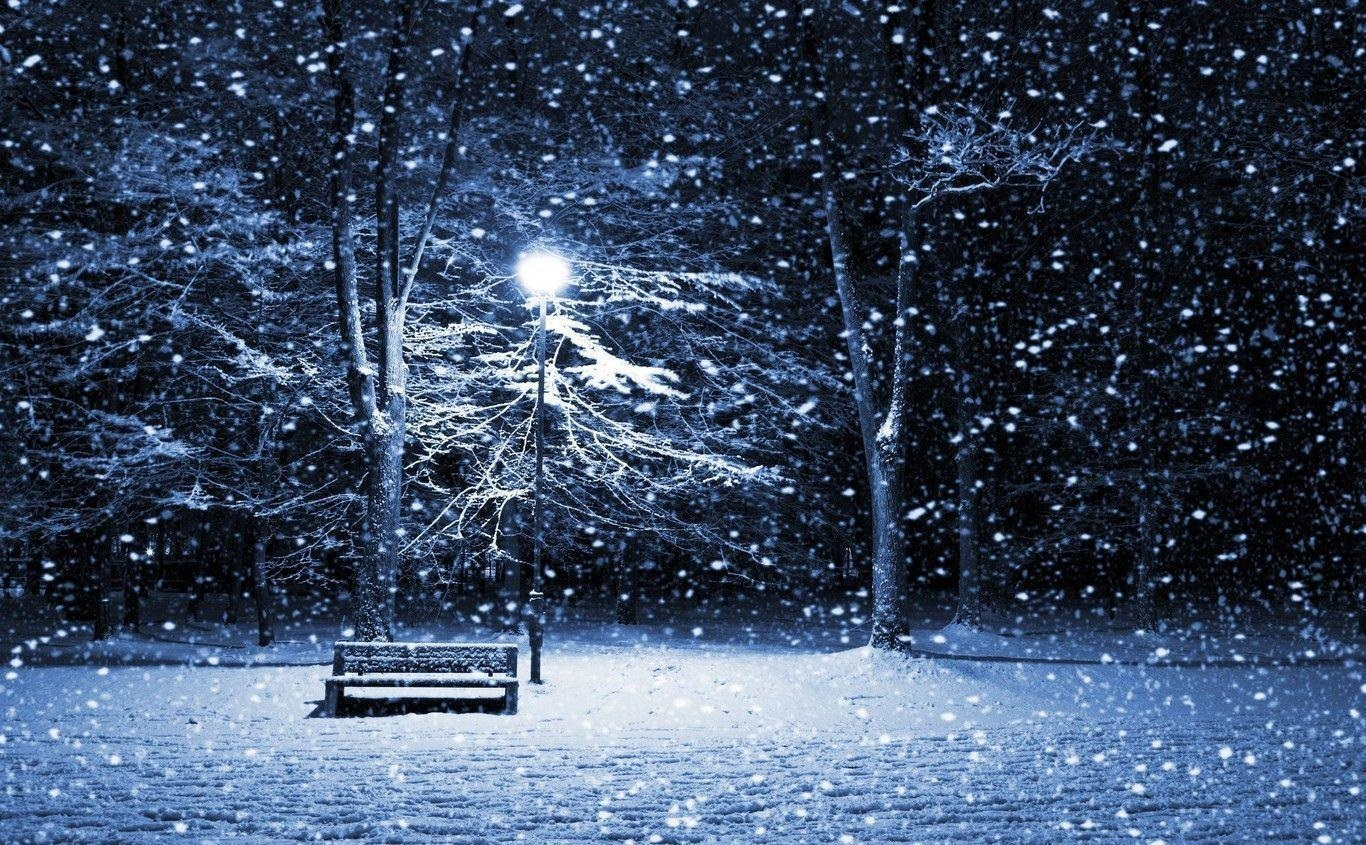
\includegraphics[width=0.4\textwidth]{Images/computer_vision/perfect_snow.jpg}
    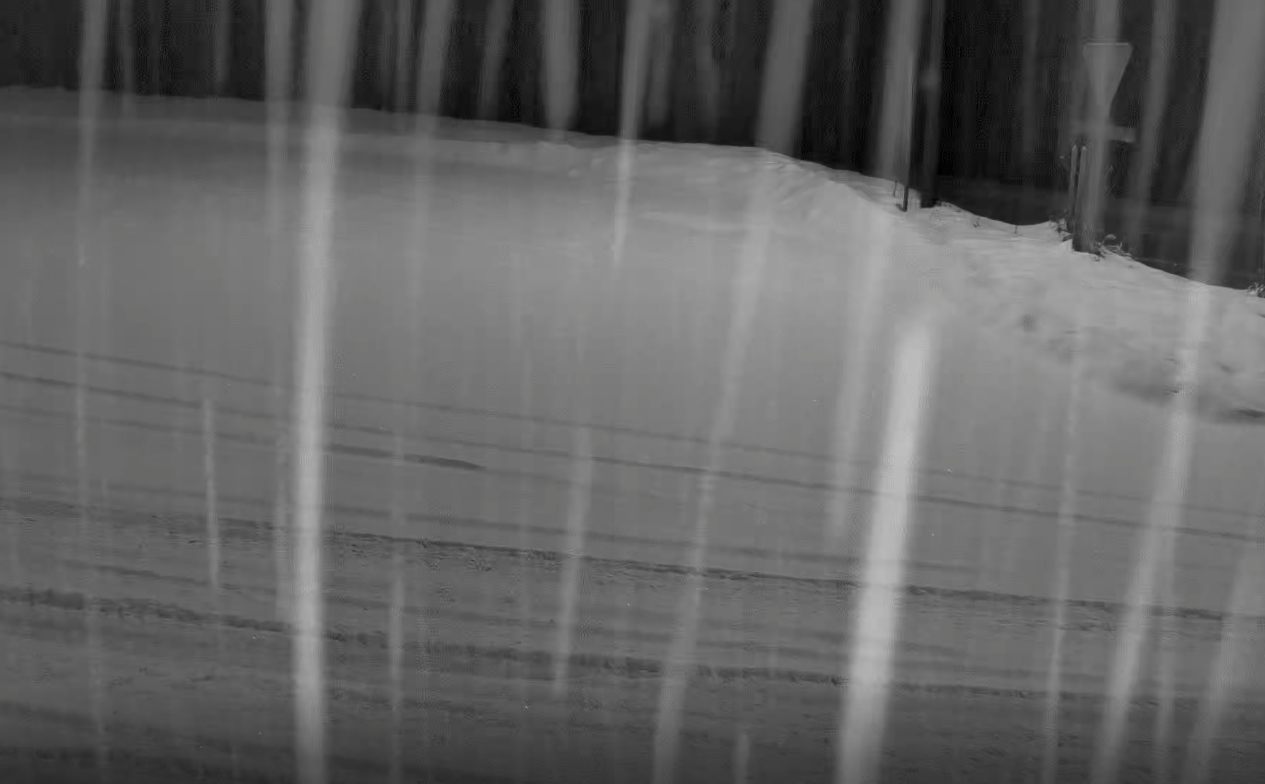
\includegraphics[width=0.4\textwidth]{Images/computer_vision/real_snow.png}
    \caption[]{Comparaison entre une image parfaite\footnotemark[1] et un cas concret\footnotemark[2]}
    \label{Snow comparison}
\end{figure}
\footnotetext[1]{\cite{PerfectSnow}}
\footnotetext[2]{\cite{VibroSnowCam}}
\newpage

\subsection{Applications pour la mesure de neige}
Les possibilités de la Computer Vision étant vaste, plusieurs méthodes ont été discutées.

\subsubsection{Mesure de niveau sur une règlette}
Les mesures de niveau de neige manuel se font déjà avec une réglette plantée dans la neige.

\begin{figure}[H]
    \centering
    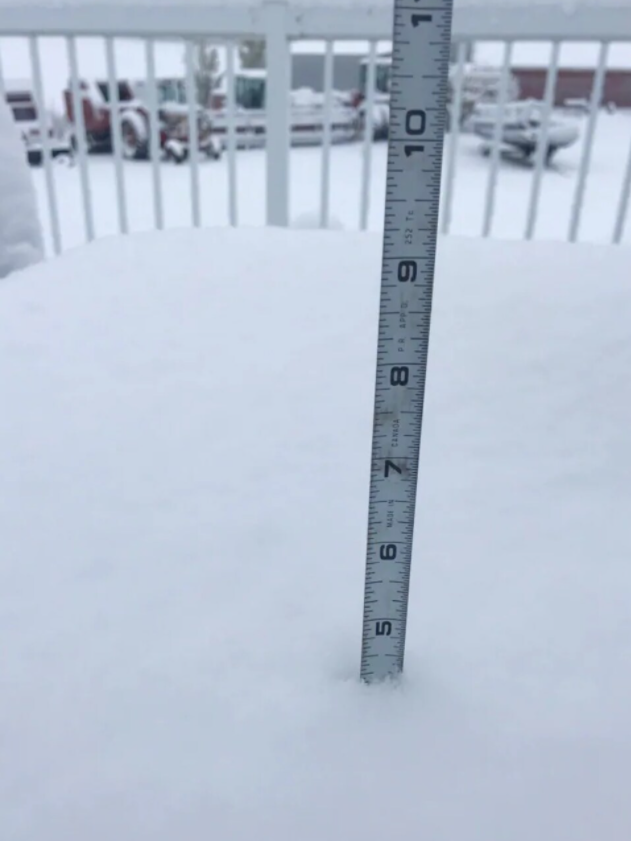
\includegraphics[width=0.4\textwidth]{Images/computer_vision/snow_meter.PNG}
    \caption[]{Mesure d'environ 4.5 pouces de neige à Manitoba, Canada\footnotemark[1]}
    \label{Snow meter}
\end{figure}
\footnotetext[1]{\cite{SnowMeter}}

La mesure pourrait être réalisé en plaçant la caméra en face de la règlette.
Deux méthodes sont possibles :
\begin{itemize}
    \item Avoir une règlette graduée, et compter le nombre de graduation encore visible
    pour déterminer la hauteur de neige.
    \item Avoir un piquet d'une taille connue, comparer la hauteur de ce piquet au nombre
    de pixel quand il n'y a pas de neige, puis mesurer le nombre de pixel non-enseveli pour
    mesure la hauteur de neige.
\end{itemize}

Cependant cette méthode présente plusieurs désavantages :
\begin{itemize}
    \item Il faut déneiger devant la caméra et la règlette, demandant probablement à un ouvrier
    de descendre de son chasse-neige pour déneiger l'installation.
    \item L'installation ne doit pas être trop proche d'une route, de risque d'être ensevelie
    ou endommagée lors du passage d'un chasse-neige.
    \item Si on utilise une règlette graduée, il faut s'assurer d'avoir un matériau
    surlequel la neige ne colle pas ou ne réfléchis pas trop la lumière du soleil.
    \item L'utilisation d'un piquet peut demander l'usage d'une intelligence artificielle
    \footnotemark[2] pour reconnaitre le piquet d'autres objets (p. ex.: arbres, lampadaires, ...).
    Cela demanderait trop de puissance de calcul pour un système embarqué basse consommation.
\end{itemize}
\footnotetext[2]{\cite{SnowTimeLapse}}
\newpage

\subsubsection{Mesure de niveau par Stéréovision}

\subsubsection{Mesure du débit de chute de neige}

\subsubsection{Détection de route enneigée}

\subsubsection{Implémentation}

